\documentclass[../main.tex]{subfiles}
%\graphicspath{{\subfix{../images/}}}

\newcommand\sbWidth{\textwidth} %Use this to set the width of all images simultaneously!

\begin{document}
\section{Problem Solving Approach}\label{finalDesign}
Prior research into the topic of alternatively powered aircraft has shown great viability in the area of electric aircraft, especially within the areas of short-haul cargo logistics. Right-on-time supply chain architecture, especially in areas of e-Commerce has created a demand for quick, efficient package distribution networks. As a result, major logistic carriers see electric aircraft as a viable option to satisfy both the consumer and their sustainability goals.It is also evidently clear that both package carriers and airports do not retain internal resources capable of designing such an infrastructure system for electric aircraft that maintains consistency and viability during the lifetime of the system.\par
With the results from the reviewed literature in consideraiton, a few solution paths were considered. These solutions were entered into a Decision Matrix seen in Figure \ref{fig:decisionMatrix}, which helped to guide our final solution. The following page shows the resultant selection matrix indicating the best (green) and worst (red) solutions. Scores for each category were aggregated via simple mean value between independent team member assessment.\par
For easy reference in the solution matrix, below can be found a short description of each solution:
\begin{singlespace}
\begin{description}
    \item[Solution \#1:] A privatized aircraft hangar supplied by the customer for use by solely the customer.
    \item[Solution \#2:] Airport or FBO-owned airport hangars for use by multiple companies wishing to operate EA out of the airport.
    \item[Solution \#3:] Development of a subsidy package for local/state/federal government funding of infrastructure installation.
    \item[Solution \#4:] A distributed power generation, storage, and distribution system for charging EA.
    \item[Solution \#5:] A large-scale power generation system with capability for on-grid power transfer.
\end{description}
\end{singlespace}
\begin{figure}[ht]
  \begin{adjustbox}{addcode={\begin{minipage}{\width}}{\caption{
      Decision Matrix of Proposed Solutions
      }
      \label{fig:decisionMatrix}
      \end{minipage}},rotate=-90,center}
      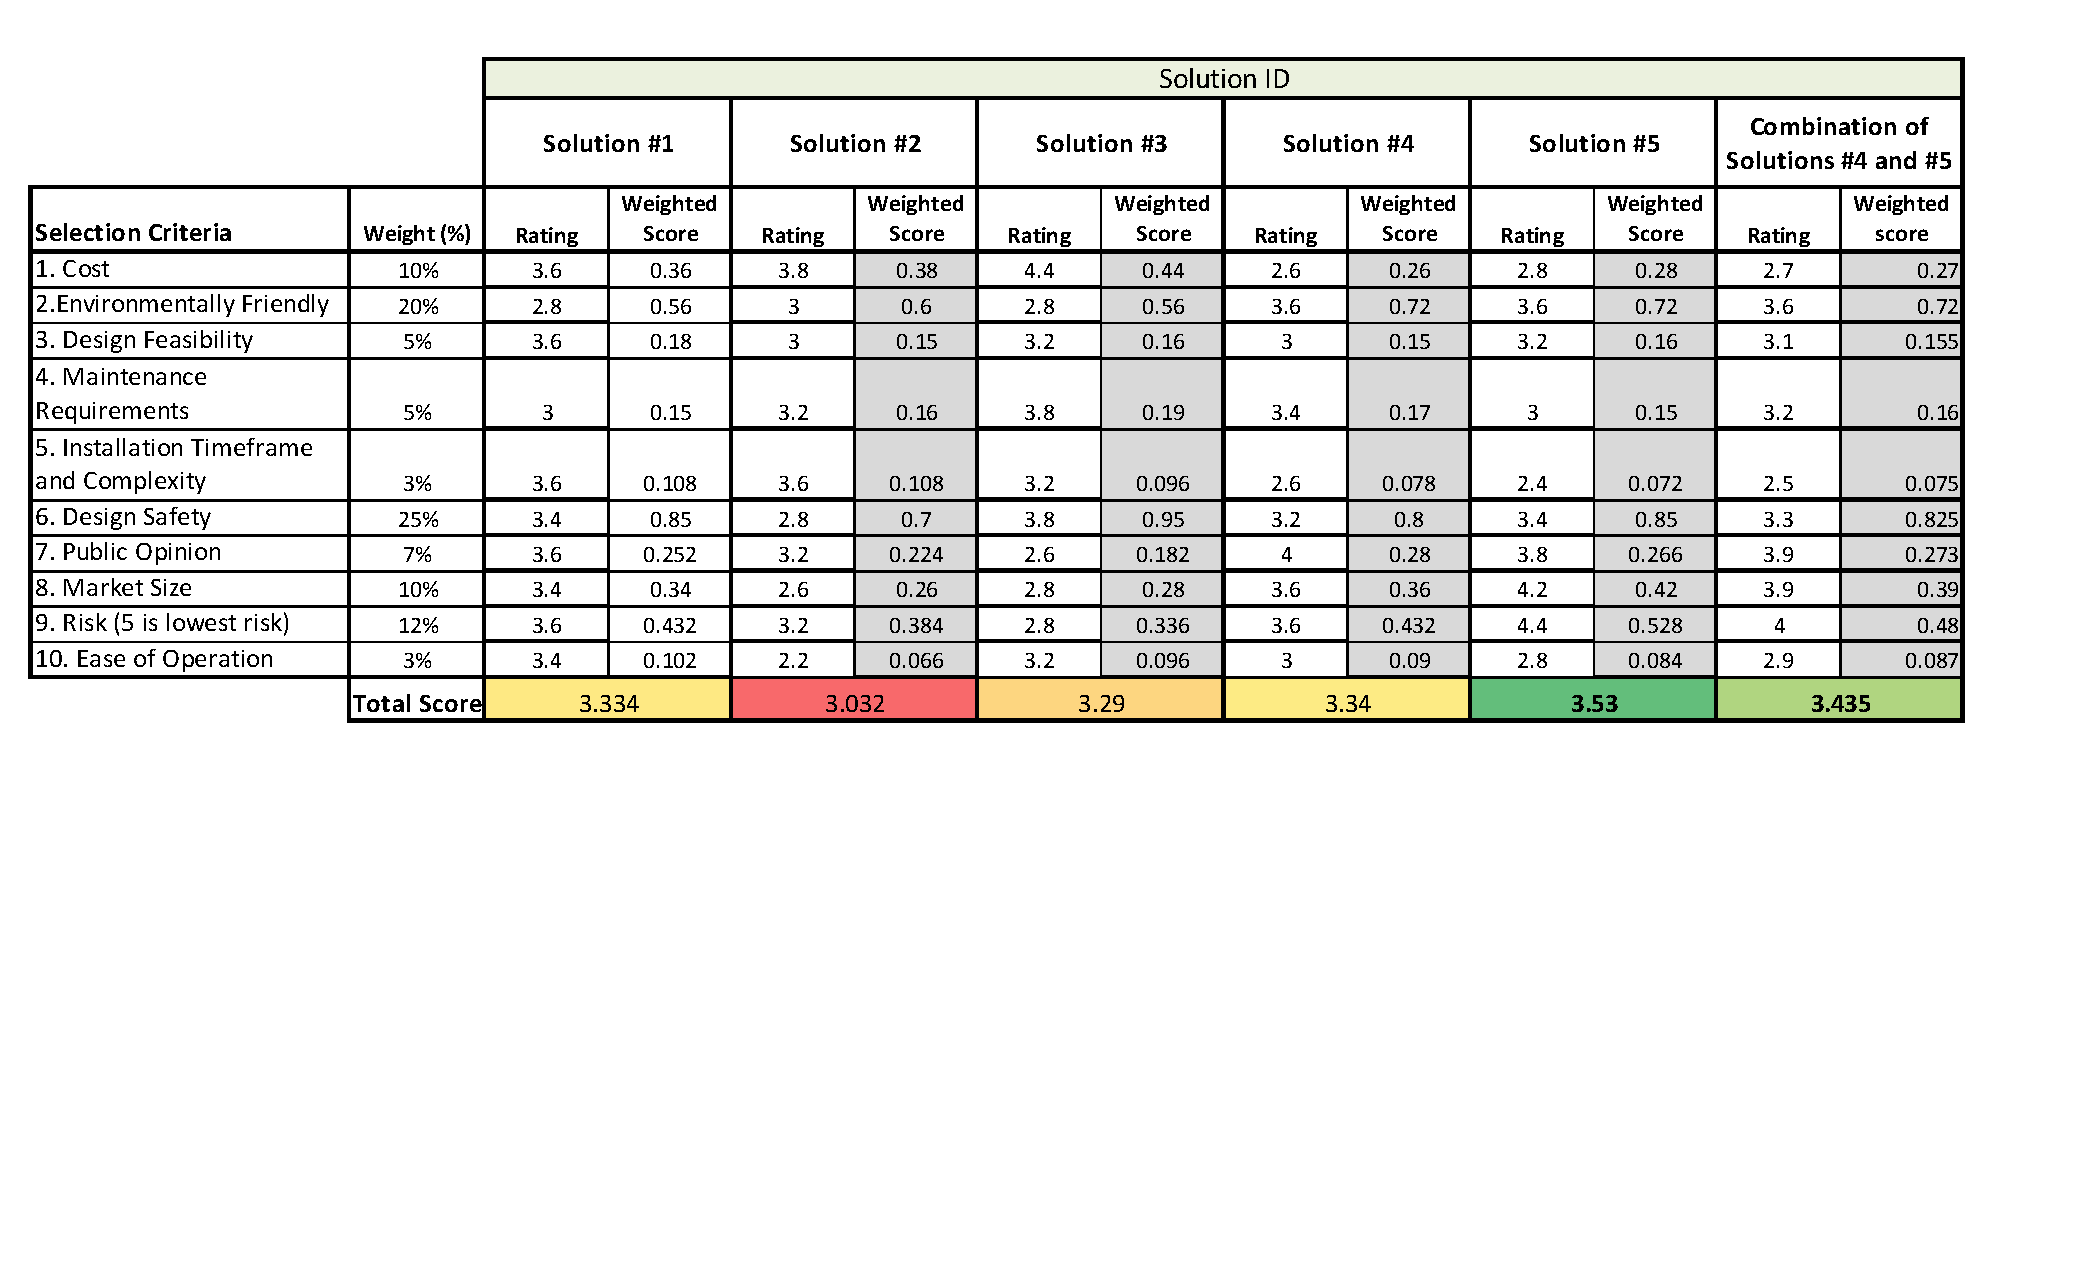
\includegraphics[scale=.6]{selectionMatrixV2.pdf}
  \end{adjustbox}
\end{figure}
\FloatBarrier
\section{System Design}
The result of this decision matrix demonstrates that the implementation of electric aircraft is a multi-faceted problem that requires many different aspects. It is also clear that considering a single element of electric aircraft does not essentially result in reliable, sustainable implementation of this new type of aircraft.\par
Our solution acts as the consultant for both airports and/or logistics companies as a system integrator for this problem. In order for such a solution involving electric aircraft to be environmentally sound, it is crucial to consider the complete infrastructure system necessary to support the new form of air transport.\par
These system elements can be broadly comprised into the following categories:
\begin{singlespace}
\begin{enumerate}
    \item Marketing of Electric Aircraft Integration
% * <Alex Stepko> 17:23:01 31 Jul 2022 UTC-0400:
% This is an awkward title, not sure what to put here.
    \item Power Generation
    \item Power Storage
    \item Power Distribution
    \item Energy Transfer to Aircraft
\end{enumerate}
\end{singlespace}

\subsection{Marketing of Electric Aircraft Integration} % MICHAEL'S SECTION
The adoption of Electric planes in the flight industry is not a question of if or how, but when. At this point in time, the addition of electric airplanes to our skies is merely a natural progression we are now witnessing and will continue to witness. This new market brings a better today along with a cleaner tomorrow by combining cheaper flights with greener transportation. In combination with a sustainable power generation source such as anti-glare solar panels, moderately frequent flights will cost virtually nothing in electricity as compared to fossil fuels. Creating green power generation will pay for itself over and over as airports continue to use this energy for their flights creating cost efficient flight affiliated fares for both the passengers and airports.\par
When discussing just the cargo and shipping capabilities, electric planes will dominate the industry. The world is constantly attracted to "faster, better, smarter" technology, and the biggest demand in the shipping world is speed. Overnight shipping, two-to-three-day shipping, you name it, every large bountiful product transport company has it. Electric planes, especially VTOL models, are ideal for not only assuring these fast and demanded services but creating a cleaner wave of transportation in the process. The most accepted form of electric aircraft are currently smaller airplanes ideal for frequent fast flights such as overnight shipment delivery, and this market segment holds massive growth capability.\par
A large benefit of green airfare is that in the event of a fuel shortage or large spike in jet fuel, electric planes will be barely affected. Because most of the "refueling" or charging process, if not all, is done naturally, electric airplanes will flourish in the event of a liquid fuel shortage or in times of hyperinflation. Airlines can offer exclusive deals, rates, and opportunities unheard of to customers through the electric plane avenue, changing the dynamic of flight fares and cargo rates.  The earlier an airport accepts and inducts these types of aircraft, the more profitable the airport will be in the near future.\par 

\subsection{Sustainable Power Generation} % ALEX'S SECTION
The concept of sustainable power generation is an inherently complex topic that in of itself can constitute a solution. However, our research has shown there is great value in providing a solution capable of performing the analysis necessary to implement a sustainable power generation system at a given site. A variety of factors contribute to the overall design, including but not limited to: climate, geography, flight throughput, maintenance costs, and the life cycle of the system. It is crucial to have a rudimentary understanding of these concepts in order to properly design the system.\par
Climate analysis is the first aspect of a power generation system. Sustainable solutions require climate that is conducive to the generational technique utilized. For example, solar generation requires climate with consistent solar radiation. Similarly, low-level solar turbines require consistent wind and weather patterns. In coastal areas, tidal generation systems may be used. However, an oceanographic survey is necessary to ensure favorable tidal patterns.\par
Once a basis for the site climate characteristics is established, it is next necessary to examine the geography available at the site. Fortunately, many airports feature large and somewhat flat land. This is primarily for safety and also gives incoming pilots an easy approach path. Sites that have a more complex terrestrial makeup constitute a more unique solution, presenting a unique set of challenges regardless of the power generation method utilized.\par
Most crucially, the system design must contain enough generation capacity. Without sufficient capacity, a sustainable solution is helpful, albeit ineffective at providing green energy to the aircraft. At existing sites, it is simple enough to perform an assessment of the cargo throughput, planes utilized, and operational schedule. These metrics can then be applied to the target electric fleet planned at the site, which results in the amount of power necessary to support that given capacity. It is advantageous to carefully consider the growth trajectory of the site when looking at throughput, as traditional cumulative growth rates may not be entirely accurate in multi-decade time frames.\par
The aforementioned assessments culminate into a site model that can be utilized in the selection of various power generation methods.

\subsection{Power Storage} % BRENDAN'S SECTION
The power storage aspect of our solution is complementary to the sustainable generation of power.  There are multiple options for storing and/or offloading the generated power that an airport must consider.\par 
%The first option is investing in large scale battery storage so that the generated electricity can be stored before an electric aircraft requires recharging. This option would be favorable for an airport that utilizes battery-swapping methods for aircraft rather than recharging-- a concept that is further detailed in the "Energy Transfer to Aircraft" section. However, this can be a costly consideration that loses efficiency as the energy is transferred between batteries. The battery technology is also still improving, so such an investment would be ineffective in the long-term.\par

% * <Alex Stepko> 19:45:11 04 Aug 2022 UTC-0400:
% Brendan, I re-worded this paragraph below. I really liked your talking points
The first and most obvious option is to invest in localized large-scale battery storage systems. These systems will store the electricity generated on-site, and will then deliver energy to the aircraft via the selected charging system. For sites that utilize a battery-swapping operational model, the batteries swapped from aircraft can be utilized as the storage elements. For a more traditional on-aircraft charging system, a separate set of batteries is necessary. This requirement can be extremely costly for a site, as the power density of current battery technology is rather low and major strides in performance are being made in this technology sector.\par
Alternatively, an airport could use its associated electrical grid as somewhat of a battery. The airport would offload it's  electricity into the grid as it is generated, and when aircraft require charging they can pull from this same grid. This option would be less viable in remote areas considering the electrical grid would have lower demand, and the transmission capabilities may already be limited. This is favorable near large cities or other areas with infrastructure demanding large amounts of electricity (i.e. refineries, factories, etc.). For more civilized areas, this storage option proves relatively low-risk, as the airport would be able to sell generated power to the grid if demand for electric aircraft is not as projected.\par

\subsection{Power Distribution} % ALEX'S SECTION

\subsection{Energy Transfer to Aircraft} % SANA'S SECTION
Once we have decided where we store this power and how we actually distribute this power, it is paramount to consider how we will transfer this energy to their aircraft using our design model. We know that traditionally, this is done by refueling with hydrocarbon fuels through a complicated network of tanks and pumps. Additionally, maintenance of the fuel distribution system is extremely expensive for an airport. With the usage of electric aircraft, airports no longer need to consider the logistics of fuel transfer. Instead, energy transfer is accomplished via battery chargers with a significantly lower operational costs.\par
Battery charging can be split into two pathways, swapping batteries and recharging batteries. Depending on specific facets of the airport, airports could adopt either model to best benefit their aircraft. First, we would consider swapping batteries. To greatly decrease turnaround time for an air frame, we would feature the capability to swap entire battery modules between planes and charging bays, eliminating the air frame’s downtime to charge batteries. This is a much more efficient solution, and the preferred one, if airports have the capacity to do so. Out-of-airframe charging with battery swaps ensures adequate cooling, charge rates, and the subsequent preservation the battery chemistry, albeit a much more technically complex infrastructure solution.\par
The other model is recharging batteries held within the airframe. This is likely the more feasible solution for airports, especially during the beginning stages of electric aircraft implementation. This would require charging stations to be set up at hangars or on designated areas of tarmac at the site. A scalable model would be built to implement these charging stations depending on the size of the aircraft, taking into consideration the anticipated fleets and operational needs. This way, aircraft could have a set road map to follow of how to implement these charging stations, no matter the size, and ensure uniform implementation across the board. With a standardized charging system available at multiple sites, a flight network soon amasses.\par
We have thought about the different ways energy can be transferred to the aircraft, and through both swapping and recharging batteries, aircraft are able to make sure their planes get the proper charge and care they need to provide energy to their trips. 

% * <Alex Stepko> 19:44:36 04 Aug 2022 UTC-0400:
% I went through and revised the first 3 lines of your writing. Great job mentioning how we have considered the many kinds of charging systems.

% * <sat5652@psu.edu> 18:06:47 04 Aug 2022 UTC-0400:
% still need to hone in on this in my section...will do tonight

This part of the solution would meet ACRP goals, specifically goal 3 which states, "Engage students at U.S. colleges and universities in the conceptualization of applications, systems and equipment capable of addressing related challenges in a robust, reliable and comprehensive manner." By thoroughly analyzing the different ways energy can be transferred to these airports, because we know not every airport can have a one size fits all solution, we have thoroughly looked at the challenge in a comprehensive manner, bringing a detailed final prototype to help combat this issue. The projected benefits of this solution would be the feasibility for any airport to implement this issue to ensure clean power generation.

\section{System Implementation}
The broad applicative nature of our solution requires a site selected for analysis. For simplicity and convenience, the University Park Airport in State College, Pennsylvania was chosen. This airport features a stable cargo and passenger throughput, and also maintains a relatively straightforward operational mode. In 2016, the University Park Airport released a \emph{Sustainable Master Plan} \cite{SCEplan} of the site detailing its operational statistics and planned improvements. The operational statistics of the airport were then utilized to develop a site model for the Risk Matrix and Cost-Benefit Analysis of this report.\par

\subsection{Safety Risk Analysis} % JADEN'S SECTION

%Jaden here's what was in the ACRP project guidelines:
%   Safety Risk Assessment: The FAA promotes a culture of safety throughout all its operations. Examine     existing FAA safety management system guidance as it relates to your proposed design solution. C      Consider inherent risks and describe how these risks should be addressed to ensure safe operations.   Be sure to reference Introduction to Safety Management Systems for Airport Operators (FAA Advisory    Circular 150/5200-37) and FAA Safety Management System Manual available under the Resources           section of the Competition website. See video with additional guidance on this section at the         Competition website

\subsection{Cost Benefit Analysis} % ALEX'S SECTION
The Cost-Benefit Analysis (CBA) of the proposed site implementation plan was developed using a thoroughly analyzed site model. This model accounts for a variety of factors; however, for simplicity sake assumptions have been made. The model makes assumptions about both the economic and technological aspects of the project, and were made in order to simplify the CBA. The assumptions are listed below, for maximum transparency into the solution's logic.
\begin{enumerate}
\begin{singlespace}
    \item Inflation rates are 0\%.
    \item The cost of electricity is constant.
    \item Solar panels remain at a fixed price, and do not decrease in performance over the life of the system.
    \item Temperate climate conducive to solar generation capacity required for the energy demands of the site.
    \item Labor rates and costs remain constant.
    \item Static depreciation of the system.
    \item Average cargo capacity of the electric aircraft utilizing the site are consistent with their traditional counterpart aircraft at the site.
\end{singlespace}
\end{enumerate}

With these assumptions made, the financial aspect of the site model can be synthesized using various resources. Our CBA accounts for enough power generation, charging, and distribution capacity to support cargo operations at the site up until approximately the year 2040, using industry-standard cumulative aggregate growth rate prediction modeling. The result of this analysis can be seen in Figure \ref{fig:CBA}.
\begin{figure}[ht]
  \begin{adjustbox}{addcode={\begin{minipage}{\width}}{\caption{
      Cost-Benefit Analysis of the University Park Airport
      }
      \label{fig:CBA}
      \end{minipage}},rotate=-90,center}
      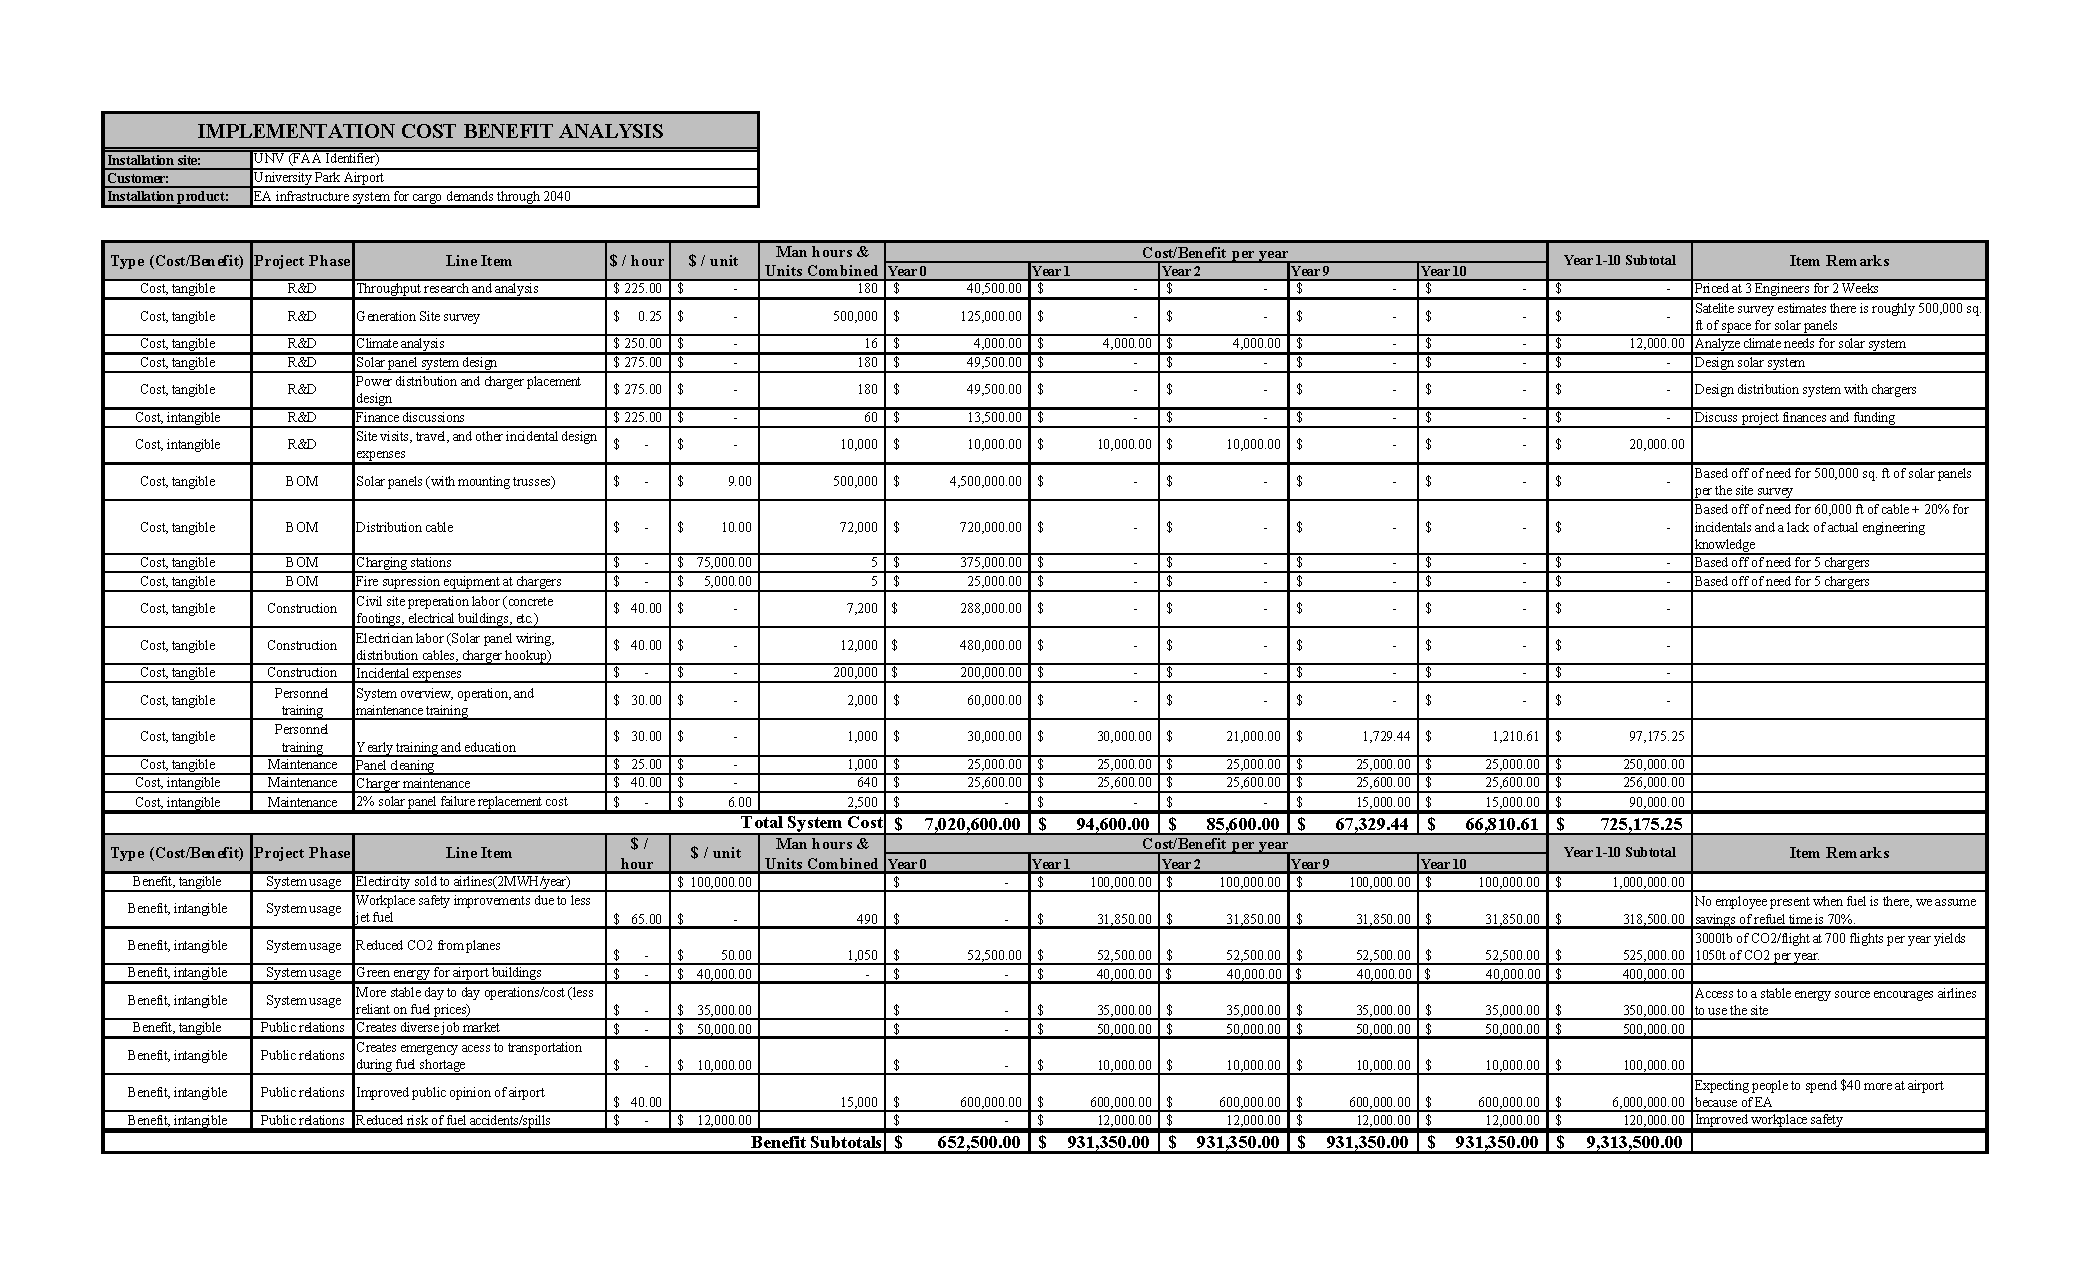
\includegraphics[scale=.6]{CBAv1.pdf}%
  \end{adjustbox}
\end{figure}
\FloatBarrier

% explain the analysis process
To describe the solution, it was necessary to outline the processes followed to develop an infrastructure solution. In prototyping, a "roadmap" was developed to satisfy this need. This piece of information roughly outlines the constituent components necessary for a sustainable infrastructure system, and can be seen below in Figure \ref{fig:roadmap}.
\begin{figure}[h!]
    \centering
    \fbox{
\includegraphics[width=6in]{roadmapV2.jpg}}
    \caption{General guidelines for the development of EA infrastructure}
    \label{fig:roadmap}
    \centering
\end{figure}
\FloatBarrier
Using this roadmap, it was first necessary to determine the terrestrial constraints of the site. Using satellite imagery and publicly available climate data, a set of constraints were determined for the site. These constraints play implications in the power generation system choice and size.\par
Next, the cargo throughput of the airport was analyzed.The University Park Airport's \emph{Sustainable Master Plan} includes cargo throughput for operation years, and also demonstrates that the airport follows the national average CAGR for cargo throughput at an airport. Notably, this shows that this site is a good indicator of the solution's implementation at other sites. Using this data, cargo capacity was extrapolated to future decades. Additionally, the carrier fleets in use at the airport were analyzed resulting in an average number of flights per day at a given cargo throughput capacity. Next, A target fleet of electric aircraft was utilized to develop a number of flights per day required to match their jet fuel counterparts. This resulted in an amount of power required per day in order to support fully sustainable operation of the electric aircraft.\par
With the result of both of these analyses, a power generation system can be selected. Low winds and ground heat capacity both indicate that wind and geothermal generation solutions are not viable for a large-capacity generation system. Solar panels hold great viability both in terms of site constraints and cargo throughput requirements. A simple survey of the terrain provides installation area for the solar panels, as seen in Figure \ref{fig:panelSites}.\par
\begin{figure}[h!]
    \centering
    \fbox{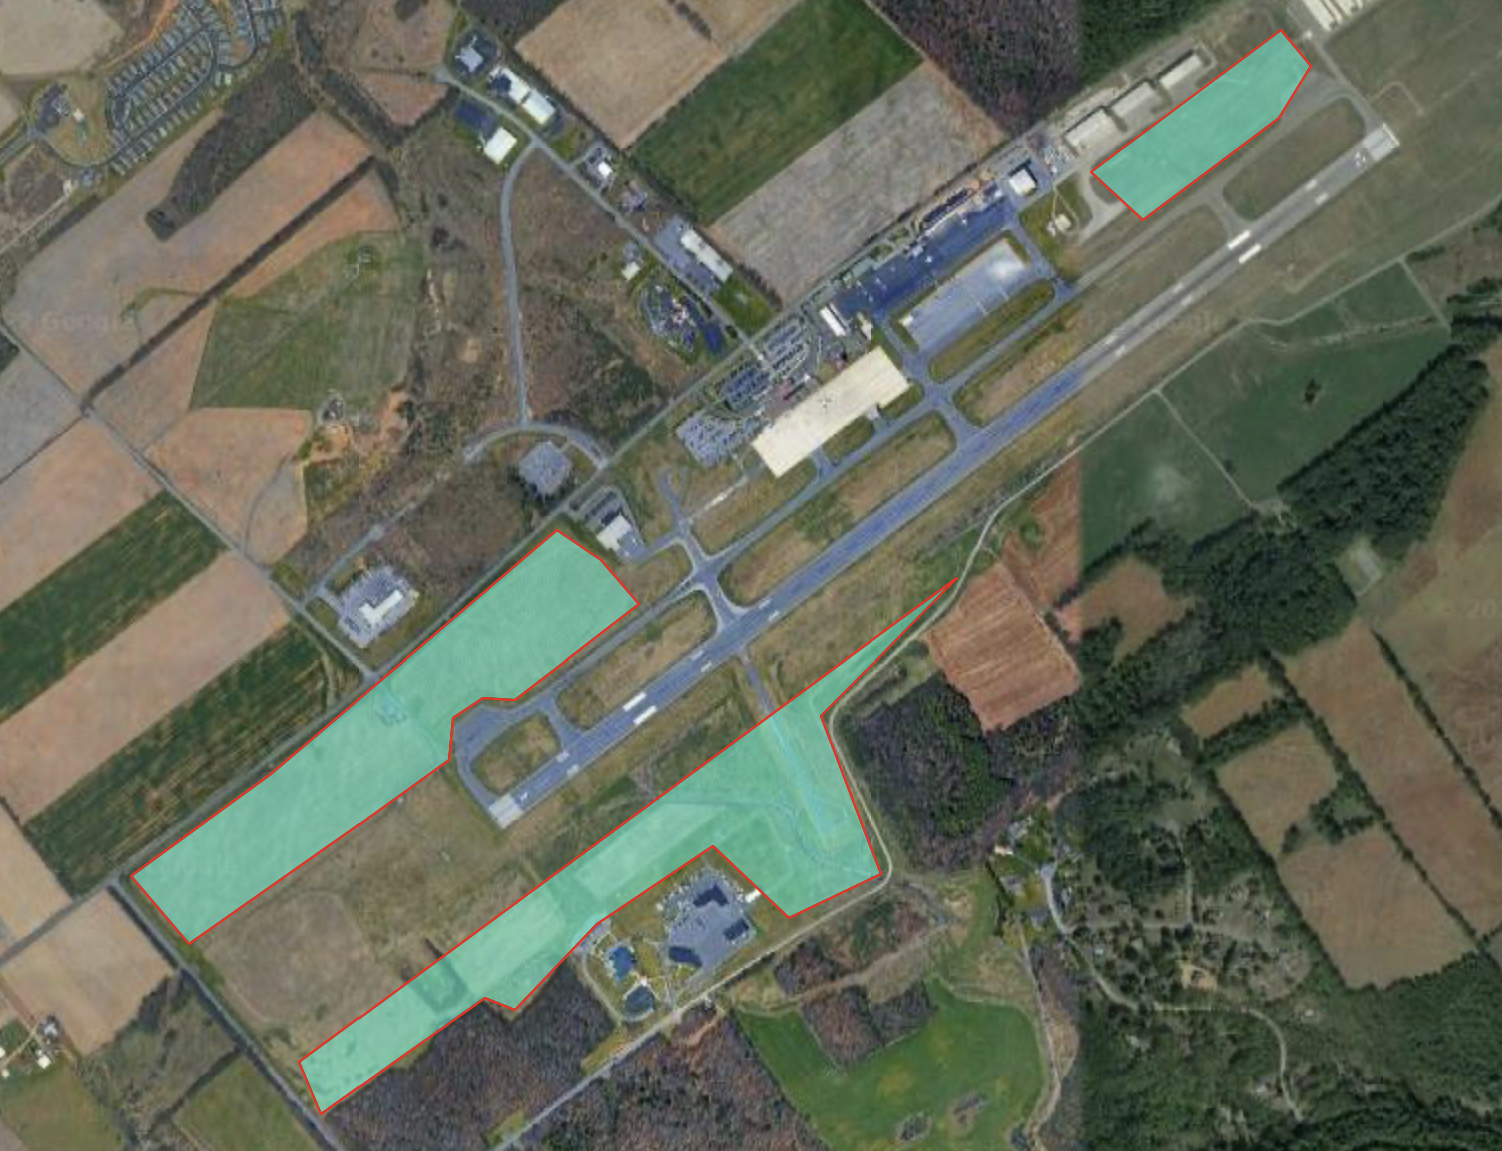
\includegraphics[width=4in]{UPSitePicture.jpg}}
    \caption{Installation site of solar panels}
    \label{fig:panelSites}
    \centering
\end{figure}
\FloatBarrier
There is approximately $500000ft^{2}$ of available space for solar panels. Low glare solar panels were selected, and approximate distribution cable lengths were determined in AutoCAD. From this amount of panel required, standard civil and electrical labor amounts were approximated.\par
Airport employees that interface with this system will require substantial training.

\end{document}